\documentclass[tikz,border=10pt]{standalone}
\begin{document}
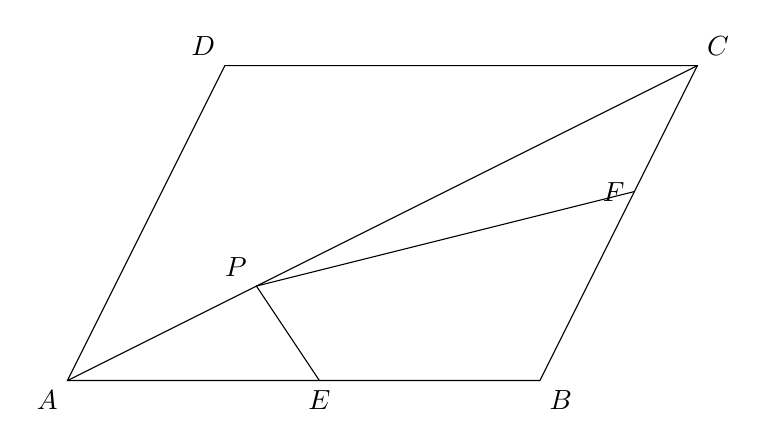
\begin{tikzpicture}
    \coordinate (A) at (0,0);
    \coordinate (B) at (6,0);
    \coordinate (C) at (8,4);
    \coordinate (D) at (2,4);
    
    \coordinate (P) at (2.4, 1.2);
    \coordinate (E) at (3.2, 0);
    \coordinate (F) at (7.2, 2.4);
    
    \draw (A) -- (B) -- (C) -- (D) -- cycle;
    \draw (A) -- (C);
    \draw (P) -- (E);
    \draw (P) -- (F);
    
    \node[below left] at (A) {$A$};
    \node[below right] at (B) {$B$};
    \node[above right] at (C) {$C$};
    \node[above left] at (D) {$D$};
    \node[below] at (E) {$E$};
    \node[left] at (F) {$F$};
    \node[above left] at (P) {$P$};
\end{tikzpicture}
\end{document}
